% Overleaf: main file is main.tex, compiler pdfLaTeX.
% biblatex uses biber, which Overleaf selects from this preamble.
% Replace the author line with your name.
\documentclass[11pt]{article}

\usepackage[margin=1in]{geometry}
\usepackage{graphicx}
\usepackage{booktabs}
\usepackage{amsmath,amssymb,amsthm}
\usepackage{placeins}
\newtheorem{theorem}{Theorem}
\newtheorem{lemma}[theorem]{Lemma}
\newtheorem{corollary}[theorem]{Corollary}
\newtheorem{proposition}[theorem]{Proposition}
\usepackage{microtype}
\usepackage[hidelinks]{hyperref}
\usepackage[backend=biber,style=numeric,sorting=none]{biblatex}
\addbibresource{references.bib}

\graphicspath{{figures/}}

\title{Pedigree-aware layout for genotype matrices\\
on opaque block storage}
\author{Author Name}
\date{}

\begin{document}
\maketitle

\begin{abstract}
Distributed genomic systems struggle with I/O efficiency when handling both biobank-wide cohort scans and selective nuclear family queries.
Opaque block storage splits a matrix into byte ranges, so a family query reads every sample packed into the blocks it opens.
We present PedPack, a pedigree-aware storage policy that searches tile width, sample grouping, and packing, and co-locates nuclear families into localized tiles when that layout wins on an opaque block engine.
We evaluate it against generic 2D tiling and the same search without pedigree identity, on simulated cohorts and on the 1000 Genomes pedigree with simulated dosages.
On moderate two-generation pedigrees the pedigree-aware search matches the exhaustive oracle ($\mathrm{fit}/\mathrm{oracle} = 1.000$) and the size-only objective is $1.20$--$1.28\times$ higher.
Held-out family reads move $16$--$18\times$ fewer bytes in the simulator, and up to $20\times$ fewer bytes on one-host HDFS in the most selective workload.
Priced per sample, a nuclear partition on two-generation pedigrees raises storage seconds by $1.08$--$1.15\times$ and lowers fit-query seconds to $0.67$--$0.85\times$.
On three-generation pedigrees the same partition still cuts a held-out family read to about $0.06\times$, but extended checks cross the partition, the fit mix pays $164$--$243$\,KB of shuffle per sample, and the query cost per sample rises, so the search keeps an all-samples layout.
The byte gap is a block-simulator result, reproduced as bytes on one machine, and again on the first 3{,}000 biallelic sites of Phase~3 chromosome~22.
There a check inside a pedigree family reads one 64\,KB block against 512\,KB for the all-samples tile, and the same rule rejects the family files when the check adds 12 people from outside the family.
The high-coverage panel of 3{,}202 samples puts the relatives back: 602 children have both parents on chromosome~22, duplication is 1.001, and a 200-site trio is one 64\,KB block against ten for the cohort.
The same check plus twelve outsiders exceeds the all-samples window.
At 128\,MB both windows are one block.
A columnar reader that can name samples does not show the Phase~3 gap: those family columns are 325 bytes.
In the large-payload limit the family layout is cheaper exactly when duplication lies below a closed threshold: \(1.387\) at a 5\% family share, \(1.080\) at a 60\% share.
Four further counts use synthetic arrivals and sit outside that cohort search.
An append-only log copies one split family in 120 bytes against a 4{,}800-byte rebuild of the same 120 people, and the retained log grows to 8{,}000 bytes because the old runs stay.
A Merkle check of 32 trio commitments returns 120 bytes on a 192-byte proof.
On an orthogonal genotype--phenotype instance the joint-query minimum switches at Mendelian fraction \(1/2\), and a query that needs only one of the two payloads prefers separate files at every fraction.
On the first 3{,}000 biallelic sites of the high-coverage chromosome~22 panel, the three columns of one real trio stitch to 9{,}000 bytes inside one 64\,KB block of a packed file of 10{,}027{,}008 bytes.
An unbuffered read of the stitch took 0.108\,ms, against 7.45\,ms for that file.
The same dosages as one Parquet row group are 15{,}069 bytes for the trio and 9{,}644{,}279 bytes for every sample.
\end{abstract}

\section{The storage problem}
\label{sec:problem}

Call the matrix $M$ variants by $N$ samples.
Hereditary checks need the child and both parents at the same loci.
Quality control and allele frequency need every sample.
In a clinical or rare-disease request the family slice is small: on the order of 5--15\% of the nuclear families in the cohort, plus, half the time, a second family that shares a parent.
The scan share of a mixed workload is the rest.

A logical tile is one sample group over a contiguous run of variants.
Tiles are packed into files.
A query reads whole tiles and rounds each file up to the block size.
If a person sits in two groups, both copies are stored and the planner reads one covering set.
On a two-generation pedigree that overlap is structural.
A person is a child in one nuclear family and a parent in the next, so a nuclear layout stores some people twice.
We call the ratio of stored sample slots to $N$ the duplication.
On our two-generation draws it sits between 1.21 and 1.30.
On three-generation draws with frequent cross-family pairing it rises to 1.42--1.44.
Co-locating every trio can still lose, because every scan pays for the extra copies.

The design is fixed before the queries arrive.
It chooses the sample groups, the variant width, the pack (\texttt{naive}, \texttt{count:$k$}, or \texttt{bytes:$B$}), and the write order (group-major or locus-major).
The score is one number, in seconds, amortized over a horizon of $H = 32$ queries:
\begin{equation}
\begin{aligned}
C(L) = {} & T_{\mathrm{build}}(L) + \omega \, S(L) \\
       & + H \bigl( 0.35 \, \overline{T}_{\mathrm{scan}}
                  + 0.40 \, \overline{T}_{\mathrm{family}}
                  + 0.25 \, \overline{T}_{\mathrm{extended}} \bigr).
\end{aligned}
\label{eq:objective}
\end{equation}
$S(L)$ is the replicated size.
$\omega$ prices the reference all-samples layout as a quarter of one reference scan.
A method that reports only selective read bytes is answering a smaller question than~\eqref{eq:objective}.

\section{What the search is allowed to see}
\label{sec:method}

Kinship follows the Karigl recursion~\cite{karigl1981}, computed in topological order and then permuted with the sample columns.
Dosages are simulated.
Founders draw two alleles.
A child inherits one allele from each parent.
The run aborts if a Mendelian check fails.
Columns are scrambled so an index-contiguous chunk is not accidentally a family.

The pool contains five groupings.
All samples in one group.
Index chunks after the scramble.
Nuclear families: two parents and their children.
Kinship agglomeration, size-capped, and a three-generation expansion that overlaps.
One fixed nuclear heuristic that does not search.
A person who belongs to two nuclear families is stored twice.
That copy is billed.

Tile bytes in the model are
\begin{equation}
\begin{aligned}
\mathrm{raw} &= \text{samples} \times \text{variants} \times \text{bytes per genotype}, \\
\mathrm{factor} &= \mathrm{clip}\bigl(0.45 \times (1 - 0.55 \times \bar\phi),\, 0.08,\, 1\bigr),
\end{aligned}
\label{eq:factor}
\end{equation}
where $\bar\phi$ is the mean kinship inside the group, off the diagonal.
The factor stands in for a codec that gets smaller on related haplotypes~\cite{durbin2014pbwt}.
It is not an implementation of PBWT.
Section~\ref{sec:codec} measures a generic codec against it.

The simulator places one task per touched file.
Replica $r$ of block $b$ in file $f$ lands on node $(h + r) \bmod n$, with $n = 8$ nodes, 64\,KB blocks, and replication 3, unless a run says otherwise.
A task runs on the live node holding the most replicas of the blocks it touches.
The rest of the read is remote.
If a query's father, mother, and child are not in one group, the model charges a shuffle of those three columns over the variant span.

The analytical model uses the same group cover and the same kinship-compressed sizes.
Its remote fraction is a formula of replication shortfall and of how many files open.
It is not a replay of task placement, so it ranks layouts well and underestimates absolute seconds.
Search uses the ranking.
On the pools below, Spearman correlation of predicted objective against measured objective is 0.95--0.99.
Mean absolute percentage error on the predicted seconds is 21--31\%.

PedPack scores every layout with that formula, measures the best $B$ of them on the simulator ($B = 36$ on the small pool, $B = 24$ on the large ones), and keeps the cheapest measured layout.
The ablation uses the same budget and the same pool.
It sees group sizes and packing.
It does not see who shares a group, it applies no kinship discount, and it treats co-location as mean group size over $N$.
Oracles are exhaustive winners inside a grouping, or over the whole pool.
They are analysis bounds.
They are not a system a user would run.
PedPack is doing its job when its fit cost matches the exhaustive winner.

Fit queries choose the layout.
Held-out family queries use different families and freshly drawn windows, and they are not in~\eqref{eq:objective}.
A ratio below 1 against the best index-chunk layout is a win on that workload.
A ratio near 1 against the full oracle means the budgeted search found the exhaustive winner.
Seeds are 7, 11, and 19 throughout.
The spread is across pedigrees, not across reruns of one draw.
A neural cost model was trained on an early run.
Its seconds error was larger than the analytical model's, and it is not part of the method.

\section{Partitioning versus cost per sample}
\label{sec:persample}

The analysis this storage is for is a hereditary check: a child and both parents, inside a window of variants.
That is three people.
On an opaque block the bytes charged are whoever else shares their blocks.
We price the two partitions the oracles picked, per person in the cohort.
Storage seconds per sample are the storage term of the fit objective divided by $N$.
Query seconds per sample are the weighted fit-query time divided by $N$.
Figure~\ref{fig:persample} is the nuclear-family oracle divided by the all-samples oracle.
The word above each group is the partition PedPack kept.

\begin{figure}[t]
  \centering
  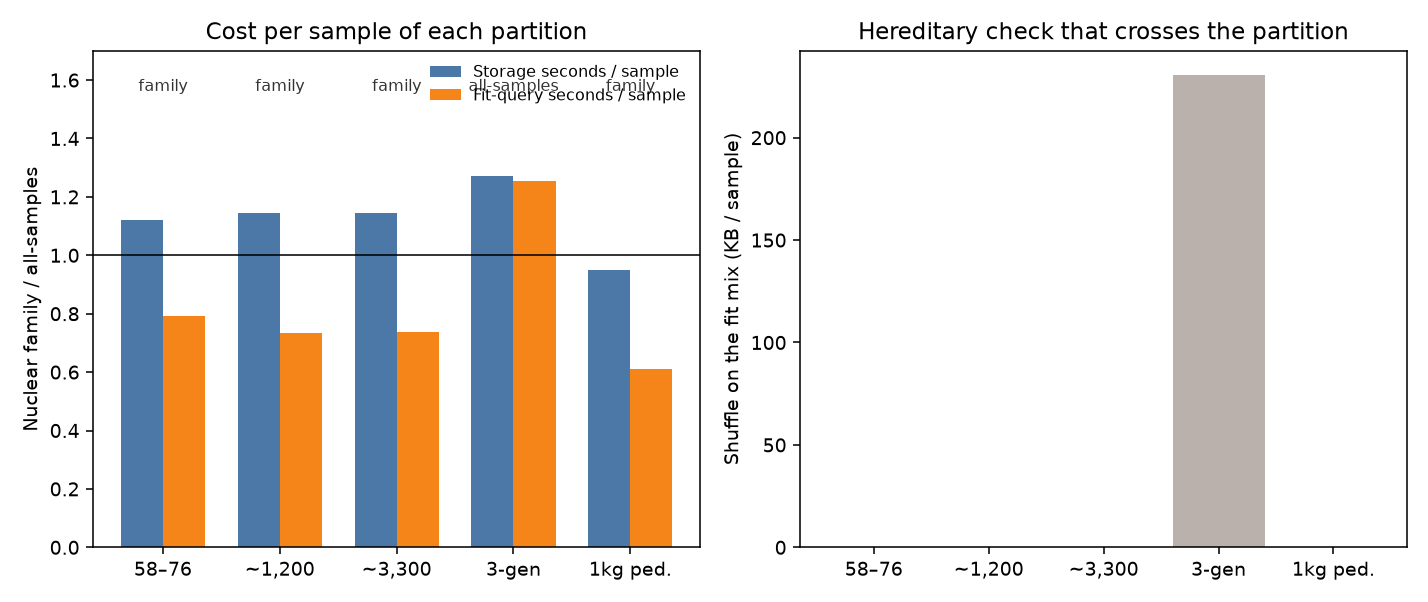
\includegraphics[width=\textwidth]{cost_per_sample.png}
  \caption{Cost per sample of a nuclear-family partition relative to one all-samples tile.
  Left: storage seconds and fit-query seconds, each divided by cohort size.
  A bar under 1 is the family partition costing less per person.
  Right: shuffle bytes per sample on the same fit mix.
  The three-generation cohort is the only one with a crossing cost, and it is the cohort where PedPack keeps all-samples.
  Held-out family bytes on that cohort are still about $0.06\times$ the all-samples read.
  The byte saving on that one check does not pay for the shuffle.}
  \label{fig:persample}
\end{figure}

On two-generation cohorts the family partition stores $1.08$--$1.15\times$ as many seconds per sample and spends $0.67$--$0.85\times$ the fit-query seconds.
The held-out check itself falls further, to $0.12$--$0.13\times$ the all-samples read at $58$--$76$ people and to about $0.06\times$ at $1{,}175$--$3{,}370$.
Shuffle on that fit mix is zero.
The nuclear groups contain the trios.

On the three-generation cohort the held-out family read is still about $0.06\times$.
Counting only that read, the extra primary bytes are smaller than the bytes one check saves, so a byte-only payback would keep the family partition.
The fit mix does not.
Extended checks cross a nuclear boundary and pay $164$--$243$\,KB of shuffle per sample.
Query seconds per sample rise to $1.10$--$1.29\times$ the all-samples layout, storage seconds per sample rise to $1.26$--$1.27\times$, and PedPack keeps all-samples.

On the 1000 Genomes pedigree, duplication is $1.001$ and shuffle is zero.
Storage seconds per sample are $0.95\times$ the all-samples layout, and query seconds per sample fall to $0.58$--$0.63\times$.
The storage dip is the model's kinship discount inside a family group together with a wider tile.
It is not a codec we measured on that pedigree.

The same locked cohorts, written to one-host HDFS, give the per-sample bill in file bytes.
Primary bytes per sample are $306$--$323$\,KB on the family files and $283$\,KB on the all-samples file.
One held-out hereditary check reads $4.0$--$5.5$\,KB per sample from the family files and $76$--$81$\,KB per sample from the all-samples file.

\section{Where family tiles win}
\label{sec:results}

\begin{figure}[t]
  \centering
  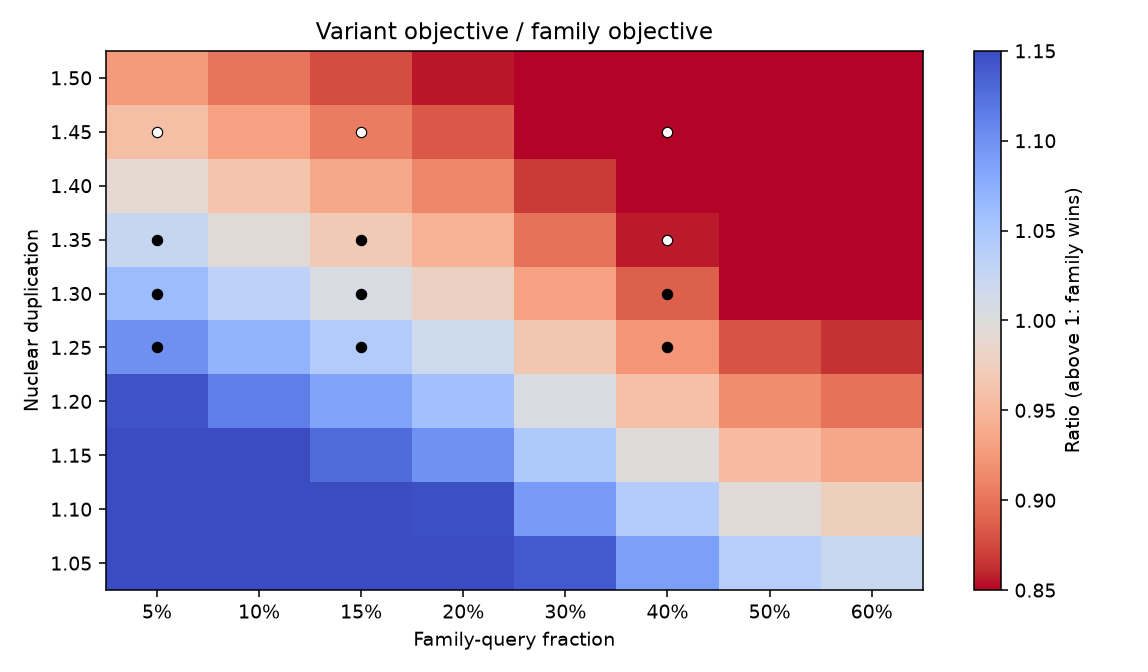
\includegraphics[width=\textwidth]{heatmap.png}
  \caption{All-samples objective divided by nuclear-family objective at 1{,}200 samples and 8{,}000 variants.
  Above 1, family tiles are cheaper.
  Both layouts are charged a remote fraction of 0.60, and neither receives the kinship compression discount.
  Black points are simulator checks in which nuclear families won.
  White points are checks in which all-samples won.
  Family tiles win on 32 of the 80 formula cells.
  The simulator agrees on the sign in 8 of 12 checks.
  The four misses are all on the boundary where the formula has already switched to all-samples and the simulator still picks families.}
  \label{fig:heatmap}
\end{figure}

Figure~\ref{fig:heatmap} is the claim with the search removed.
At duplication 1.30 and a family-query fraction of 5\% the ratio is 1.06.
At duplication 1.43 and the same fraction it is 0.97.
At duplication 1.30 and a 60\% family share it is 0.83.
Family tiles pay for themselves when queries are selective and overlap is moderate.
They lose when either knob moves far enough.

\subsection{Decision theorem}
\label{sec:inequality}

The search is a comparison of two objectives.
This subsection removes block rounding and file opens and proves when the family layout is the cheaper of the two.
The rounded model of Figure~\ref{fig:heatmap} is the check, not the proof.

Fix a cohort of \(N\) samples and \(M\) variants, a stored byte \(\sigma\) per genotype, and payload \(S = N M \sigma\) for the all-samples layout.
The family layout stores \(D S\) bytes with \(D \ge 1\).
A query mix puts weight \(\alpha\) on a full scan, \(\beta\) on a family query, and \(\gamma\) on an extended query, with \(\alpha+\beta+\gamma = 1\).
The family query names a fraction \(f \in (0,1]\) of the stored family bytes.
The extended query names \(e(f) = \min(1, 2f)\).
Selective queries touch a fraction \(w \in (0,1]\) of the variants.
The horizon is \(H\) queries.
Both layouts see the same remote fraction \(r\).
Replication is \(\rho \ge 1\).
Storage of the all-samples layout is priced at \(\eta\) of one all-samples scan.

Let \(B_{\mathrm{loc}}\) and \(B_{\mathrm{rem}}\) be the local and remote bandwidths, and let \(g\) be the genotype decode rate.
The seconds per payload byte, and the seconds to write one extra payload byte, are
\begin{align}
c_{\mathrm{byte}}
  &= \frac{1-r}{B_{\mathrm{loc}}} + \frac{r}{B_{\mathrm{rem}}} + \frac{1}{\sigma_0 \, g}, \\
c_{\mathrm{write}}
  &= \frac{1}{B_{\mathrm{loc}}} + \frac{\rho-1}{B_{\mathrm{rem}}},
\end{align}
where \(\sigma_0\) is the uncompressed record size used by the decode term.
On the bandwidths of this paper, \(r = 0.60\), \(\rho = 3\), \(\eta = 0.25\), \(H = 32\), \(w = 0.30\), and \((\alpha,\beta,\gamma) = (0.35, 0.40, 0.25)\),
the two rates are \(c_{\mathrm{byte}} = 9.625\times 10^{-9}\) and \(c_{\mathrm{write}} = 3\times 10^{-8}\).

The proof uses seven restrictions.
Both layouts share \(r\).
Kinship does not change \(\sigma\).
Queried trios lie inside the groups that are opened, so shuffle is zero.
A family query reads the fraction \(f\) of the family payload, and an extended query reads \(e(f)\).
Build reads the source matrix once for either layout.
Only the primary write and the replica writes differ.
File-open time and block rounding are omitted, which is the regime in which every read covers many blocks.

\begin{lemma}[Block transfer]
\label{lem:blocks}
A contiguous read of \(L\) bytes on block size \(B\) moves \(\lceil L/B \rceil\) blocks.
For an all-samples window \(L_{\mathrm{all}} = N W \sigma\) and a group window \(L_{\mathrm{grp}} = g W \sigma\), the block ratio is \(\lceil L_{\mathrm{all}}/B \rceil / \lceil L_{\mathrm{grp}}/B \rceil\).
\end{lemma}

\begin{proof}
The store returns a whole block for every block the byte range touches, so the transfer length is the smallest multiple of \(B\) that covers \(L\).
The ratio is that count for the cohort window divided by that count for the group window.
\end{proof}

\begin{lemma}[Many-block limit]
\label{lem:limit}
Let the family read be the fraction \(f D\) of the all-samples window, with \(f D > 0\).
As both payloads tend to infinity the block ratio tends to \(1/(f D)\).
\end{lemma}

\begin{proof}
\(\lceil x \rceil = x + \theta\) for some \(\theta \in [0,1)\).
The ratio of two such terms tends to the ratio of the payloads, which is \(1/(f D)\).
\end{proof}

\begin{theorem}[Family layout is cheaper below a duplication threshold]
\label{thm:gap}
Under the seven restrictions above, write
\begin{align}
A(f) &= c_{\mathrm{write}} + \eta\, c_{\mathrm{byte}}
  + H c_{\mathrm{byte}} \bigl(\alpha + w(\beta f + \gamma e(f))\bigr), \\
K &= c_{\mathrm{write}} + \eta\, c_{\mathrm{byte}}
  + H c_{\mathrm{byte}} \bigl(\alpha + w(\beta + \gamma)\bigr).
\end{align}
Then \(A(f) > 0\), and the family objective is strictly smaller than the all-samples objective if and only if \(D < K / A(f)\).
\end{theorem}

\begin{proof}
The all-samples scan moves \(S\) bytes and the family scan moves \(D S\).
A selective all-samples read moves \(w S\).
The matching family and extended reads move \(f D S\) and \(e(f) D S\) after the window fraction is applied to the stored family payload, which contributes the factors \(w f D\) and \(w e(f) D\) against \(w\).
Seconds are \(c_{\mathrm{byte}}\) times bytes because \(r\) is shared and shuffle is zero.
One query therefore differs by \(c_{\mathrm{byte}} S\, Q(D,f)\), where
\[
Q(D,f) = \alpha(D-1) + w\beta(f D - 1) + w\gamma\bigl(e(f) D - 1\bigr).
\]
Over the horizon the query gap is \(H c_{\mathrm{byte}} S\, Q(D,f)\).

Build reads the same source matrix either way.
The family layout writes \((D-1)S\) extra payload bytes, the primary at local bandwidth and \(\rho-1\) replicas at remote bandwidth, which is \((D-1) S\, c_{\mathrm{write}}\).

The storage price of a layout is \(\eta\) times the all-samples scan, scaled by that layout's payload.
In this limit the all-samples scan is \(c_{\mathrm{byte}} S\), so the storage gap is \(\eta c_{\mathrm{byte}} (D-1) S\).

Add the three gaps and divide by \(S > 0\):
\begin{equation}
\frac{C_{\mathrm{fam}} - C_{\mathrm{all}}}{S}
  = (D-1)\bigl(c_{\mathrm{write}} + \eta c_{\mathrm{byte}}\bigr) + H c_{\mathrm{byte}}\, Q(D,f).
\label{eq:gap}
\end{equation}
Expand \(Q\).
The coefficient of \(D\) is \(A(f)\), and the remaining terms are \(-K\), so the right-hand side equals \(A(f)\, D - K\).
Every term in \(A(f)\) is non-negative and \(c_{\mathrm{write}} > 0\), so \(A(f) > 0\).
The family objective is smaller exactly when \(A(f)\, D - K < 0\), that is \(D < K/A(f)\).
\end{proof}

\begin{corollary}
\label{cor:thresholds}
On the rates above, the threshold \(K/A(f)\) is \(1.387\) at \(f = 0.05\), \(1.312\) at \(f = 0.15\), \(1.154\) at \(f = 0.40\), and \(1.080\) at \(f = 0.60\).
\end{corollary}

\begin{proof}
Substitute \(c_{\mathrm{byte}}\), \(c_{\mathrm{write}}\), \(\eta\), \(H\), \(w\), and \((\alpha,\beta,\gamma)\) into \(A(f)\) and \(K\).
For \(f \le 1/2\), \(e(f) = 2f\).
For \(f = 0.60\), \(e(f) = 1\).
The four quotients are the stated values.
At those parameters the left side of \eqref{eq:gap} equals zero when \(D = K/A(f)\).
\end{proof}

The threshold sits between the two duplication cells already plotted.
At \(D = 1.30\) and \(f = 0.05\), which is below \(1.387\), the left side of \eqref{eq:gap} is \(-1.26\times 10^{-8}\) and the rounded model ratio is \(1.06\).
At \(D = 1.43\) and \(f = 0.05\), above the threshold, it is \(+6.17\times 10^{-9}\) and the ratio is \(0.97\).
At \(D = 1.30\) and \(f = 0.60\), above \(1.080\), it is \(+4.09\times 10^{-8}\) and the ratio is \(0.83\).
On the \(16\times 12\) grid from \(D = 1.00\) to \(1.75\) and \(f = 0.05\) to \(0.60\), Theorem~\ref{thm:gap} has the same sign as the rounded model on 190 of 192 cells.
The two misses have rounded ratios \(0.995\) and \(0.998\).

Lemma~\ref{lem:blocks} fixes the public window before the limit is taken.
A 200-site window of 2{,}504 one-byte dosages is 8 blocks of 64\,KB against 1 block for a pair, and 1 block against 1 block at 128\,MB.
The scaled stored genotype is \(400 \times 0.45 = 180\) bytes.
A 2{,}400-variant window of 1{,}200 samples is 4 blocks of 128\,MB, and 5\% of a layout at duplication \(1.30\) is 1 of those blocks, a ratio of 4.
Lemma~\ref{lem:limit} gives \(1/(0.05 \times 1.30) = 15.4\) once both reads are large.
At 100{,}000 variants the same fraction is 161 blocks against 11, a ratio of \(14.6\).

\begin{figure}[t]
  \centering
  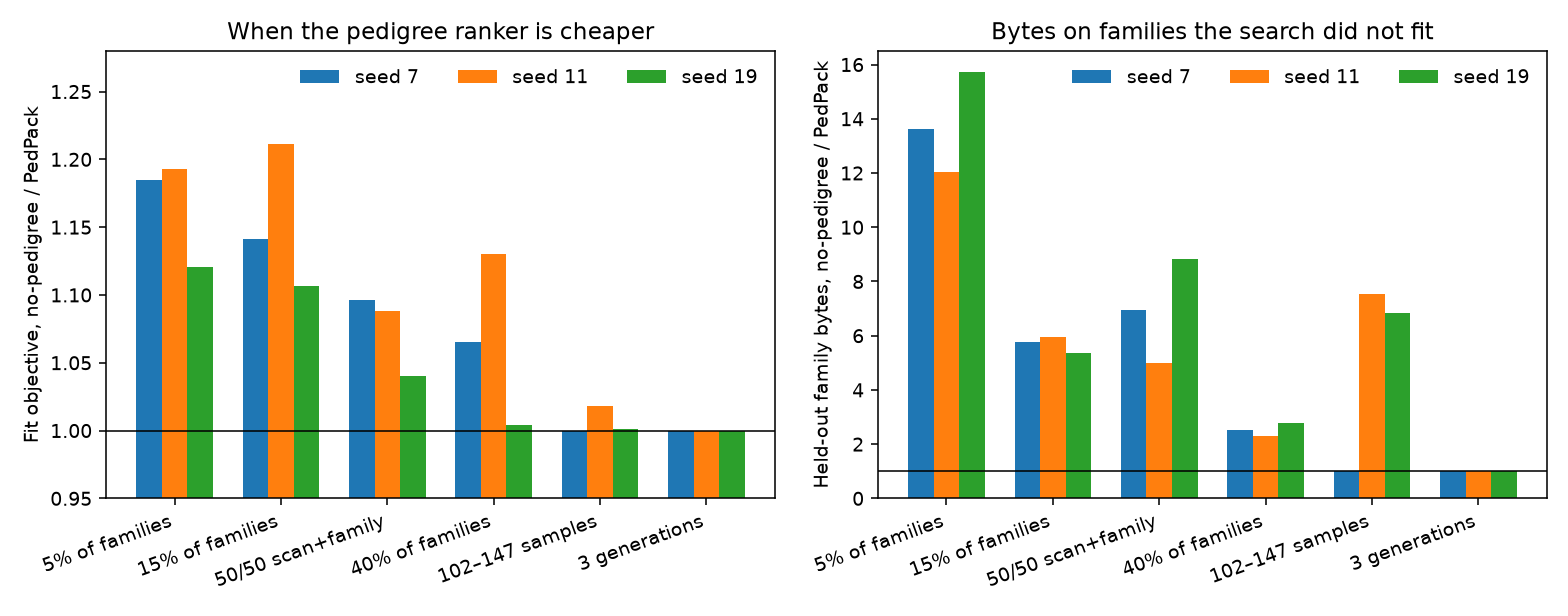
\includegraphics[width=\textwidth]{regimes.png}
  \caption{The same search, re-run under one change at a time.
  Left: fit objective of the size-only ranker divided by PedPack.
  Right: held-out family bytes, same ratio.
  A bar at 1 means the two rankers chose layouts of equal measured cost.
  On two-generation pedigrees the pedigree ranker stays ahead from a 5\% family share through a 50/50 scan mix.
  At three generations and a cross rate of 0.6 the ratio falls to 1 and both rankers select all-samples.}
  \label{fig:regimes}
\end{figure}

The search follows that surface.
On a locked two-generation cohort of 58--76 people and 1{,}600 variants, PedPack selects nuclear families on every seed and matches the full oracle.
The size-only ranker selects all-samples.
Median fit cost of the family layout is 0.286$\times$ the best index-chunk layout.
An earlier configuration, 48 bytes per genotype, 256\,KB blocks, and a heavier scan share, does not produce this split.
Both rankers stay on all-samples.
That run is a different workload.
We do not mix it into Table~\ref{tab:cohorts}.

Figure~\ref{fig:regimes} moves one factor at a time.
At 5\%, 15\%, and 40\% of families, and on a fit mix that is half scans, the two rankers still pick different layouts and the pedigree choice is cheaper.
At 40\% the objective ratio on one seed shrinks to 1.004, while held-out bytes stay 2.3--2.8$\times$ apart.
Three generations and a cross rate of 0.6 push duplication to 1.33--1.45.
Both rankers then select all-samples, and the family oracle costs more than the variant oracle (6.34 against 5.01, 4.73 against 4.04, and 6.61 against 5.29 on the three seeds).
Cutting the scan share from 0.35 to 0.20 restores a family choice on one seed only.
A larger three-generation draw, 102--147 people and 3{,}200 variants, is the same story: the seed at duplication 1.45 picks all-samples; the other two pick families with fit ratios 1.018 and 1.001.
The search does not prefer families.
It prefers the cheaper layout.

\begin{table}[t]
  \centering
  \caption{What each ranker selects.
  The fit ratio is the size-only objective divided by the PedPack objective.
  On the overlap row both rankers select all-samples, so the ratio is 1.
  On the 1000 Genomes row both select a family-sized grouping and their objectives agree to within 0.2\%.}
  \label{tab:cohorts}
  \begin{tabular}{@{}llrrrr@{}}
    \toprule
    Cohort & People & Dup. & PedPack & Size-only & Fit ratio \\
    \midrule
    Locked, 2 gen. & 58--76 & 1.21--1.27 & family & all-samples & 1.11--1.18 \\
    Scale, 2 gen. & 1{,}175--1{,}207 & 1.28--1.30 & family & all-samples & 1.20--1.28 \\
    Scale, 2 gen. & 3{,}328--3{,}370 & 1.293--1.298 & family & all-samples & 1.21--1.24 \\
    Overlap, 3 gen. & 667--685 & 1.42--1.44 & all-samples & all-samples & 1.00 \\
    1000 Genomes & 3{,}375 & 1.001 & family-sized & family-sized & $< 1.002$ \\
    \bottomrule
  \end{tabular}
\end{table}

Table~\ref{tab:cohorts} is the same split at two larger sizes.
At 1{,}175--1{,}207 people and 8{,}000 variants, held-out family bytes on the all-samples layout are 16.3--17.6$\times$ the family layout.
Scan bytes go the other way, 1.15--1.17$\times$, because the overlapping parents are stored twice.
The family layout costs more to build (76--79\,s against 70--71\,s) and more to store (4.7--4.9\,s against 4.2--4.3\,s).
Query time is where it wins (4.4--5.9\,s against 6.5--7.8\,s).

\begin{figure}[t]
  \centering
  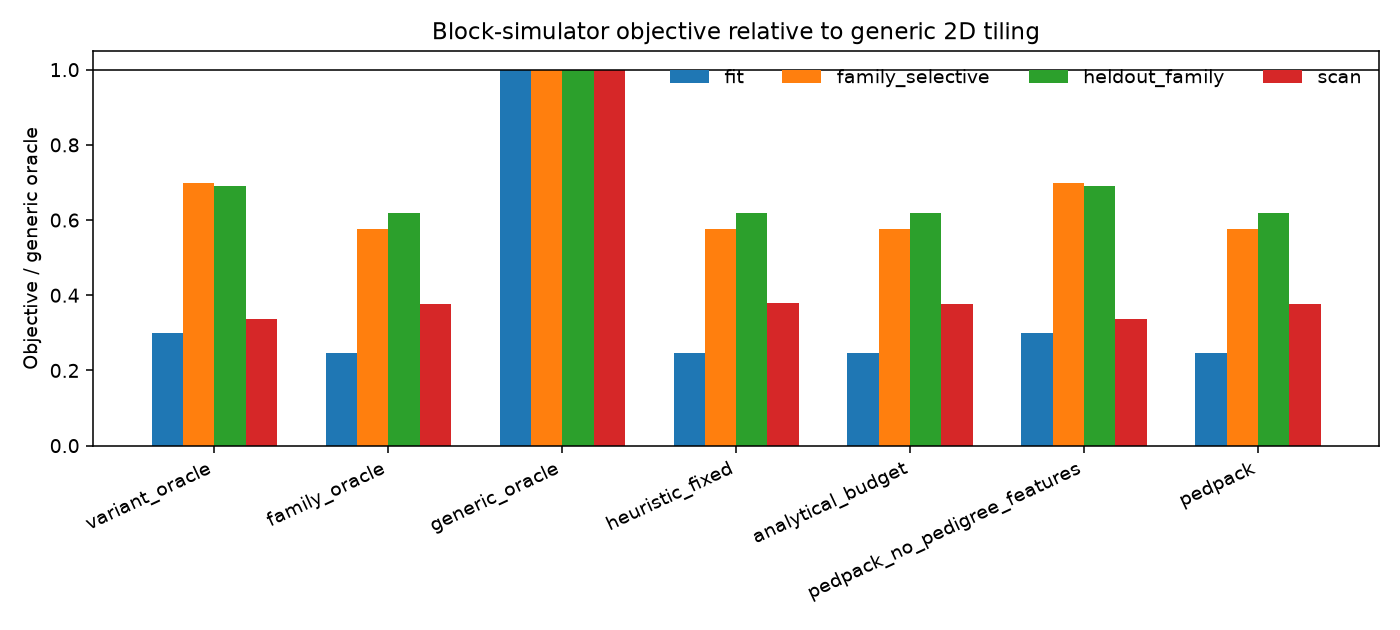
\includegraphics[width=0.92\textwidth]{scale3k.png}
  \caption{Block-simulator objective relative to the best index-chunk layout, median over seeds, at 3{,}328--3{,}370 people and 8{,}000 variants.
  PedPack matches the family oracle and the exhaustive winner.
  The ranker that cannot see who shares a group matches the all-samples oracle.
  Index chunks remain the expensive layout because split trios pay a shuffle the family groups do not.}
  \label{fig:scale3k}
\end{figure}

At 3{,}328--3{,}370 people the split does not move (Figure~\ref{fig:scale3k}).
Duplication is 1.293--1.298.
Fit ratios are 1.244, 1.211, and 1.208.
Held-out family bytes are 16.8$\times$, 17.3$\times$, and 16.7$\times$.
Build and storage are again higher for families (217--220\,s and 13.4--13.6\,s, against 197--199\,s and 11.8--11.9\,s).
Query time is lower (14.7--17.5\,s against 20.0--23.5\,s).
The split at about 3{,}300 people is the split at about 1{,}200.
What closes it is duplication, on the three-generation draw in Figure~\ref{fig:overlap}.

\begin{figure}[t]
  \centering
  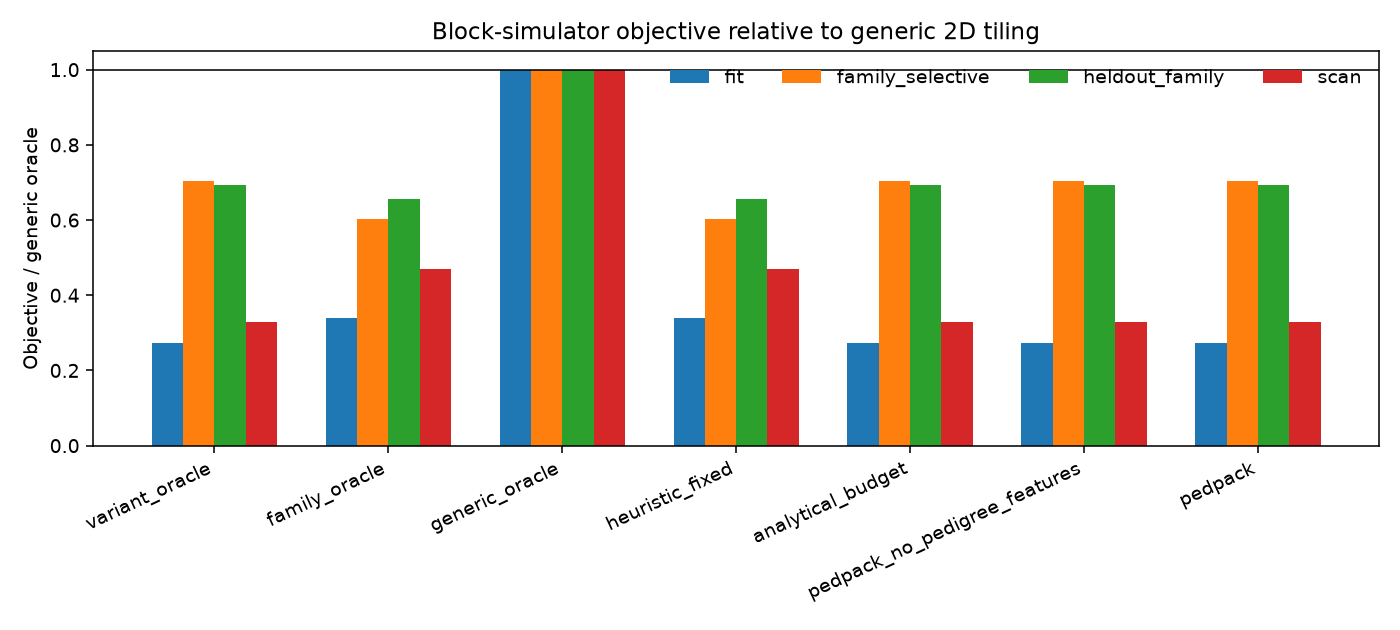
\includegraphics[width=0.92\textwidth]{overlap.png}
  \caption{The closed side of the boundary at the same variant count: 667--685 people, three generations, cross rate 0.6, family-oracle duplication 1.42--1.44.
  PedPack and the size-only ranker select the same all-samples layout and match the variant oracle.
  The family oracle is more expensive.
  On seed 7 its fit objective is 218.7 against 173.1 for all-samples.}
  \label{fig:overlap}
\end{figure}

The 1000 Genomes phase~3 pedigree~\cite{genomes2015} is the same selector on a public graph.
We keep the 3{,}375 people who have both parents recorded or neither: 636 children and 2{,}739 founders.
Dosages are still simulated.
Nuclear duplication is 1.001.
There is almost no overlapping membership.
Both rankers reject all-samples, and their fit objectives agree to within 0.2\% on every seed.
All-samples remains expensive: its fit objective is 1.42$\times$, 1.43$\times$, and 1.49$\times$ PedPack, and it reads 20.1$\times$, 18.6$\times$, and 19.9$\times$ more bytes on held-out families.
When groups barely overlap, group size is enough for both rankers to leave the single all-samples tile.
Figure~\ref{fig:overlap} is the other side of that: overlap is high, and both rankers keep all-samples.

\FloatBarrier
\section{A codec check, then real readers}
\label{sec:codec}

Zstandard level 3, on 800-variant haplotype tiles, compresses a nuclear family to 0.907$\times$ an equal-sized founder tile on the locked seeds and to 0.918$\times$ at 1{,}175--1{,}207 people.
Equation~\eqref{eq:factor} predicts 0.883 and 0.888 at the same mean kinship.
The relative discount is in the right direction and within a few points of this codec.
The absolute 0.45 is not the measured Zstandard-to-raw ratio, which is about 0.17 on these one-byte alleles.
That constant still prices the opaque 400-byte genotype used in the simulator.
This is not a PBWT measurement.

\begin{table}[t]
  \centering
  \caption{Readers other than the simulator.
  HDFS is one host, Hadoop 3.2.1, replication 3, 64\,KB blocks.
  Byte ratios are all-samples over the family layout on held-out families.
  Hail and Parquet are local and columnar.
  They do not reproduce the block-store gap.}
  \label{tab:systems}
  \begin{tabular}{@{}llr@{}}
    \toprule
    Reader & What was compared & Result \\
    \midrule
    HDFS, 5\% families & padded tiles, 3 seeds & byte ratio 14.2--20.2 \\
    HDFS, 15\% families & same & 6.5--6.9 \\
    HDFS, 50/50 mix & same & 5.8--10.5 \\
    HDFS, 3-gen.\ overlap & both rankers chose one layout & ratio 1.0 \\
    Hail, 361 tables & seed 7, 1{,}207 $\times$ 8{,}000 & scan 169\,s vs.\ 0.55\,s \\
    Parquet, 12 files & seed 7, \texttt{count:32} & held-out bytes tied \\
    Parquet, 1 file & same columns, one footer & 0.063\,s vs.\ 0.106\,s \\
    \bottomrule
  \end{tabular}
\end{table}

Table~\ref{tab:systems} is the transfer off the simulator.
The HDFS files are the layouts the simulator chose, padded out to the modeled tile size, with no codec.
The client is not a DataNode, so every block is remote.
That is not the simulator's remote-read fraction.
On the selective two-generation layouts the family files return fewer bytes, touch fewer blocks, and finish sooner.
On \texttt{select\_05} the three seeds use 72.3, 53.2, and 64.9\,MB of replicated space with the family layout, against 64.6, 49.4, and 56.9\,MB for all-samples.
On the three-generation overlap regime both rankers had chosen all-samples, and the NameNode serves the same bytes.
This is real HDFS~\cite{shvachko2010hdfs}.
It is one machine: one NameNode and three DataNodes in Docker on a single host.

Hail 0.2.139~\cite{hail} in Spark local mode does not reproduce the gap, and the way it fails is informative.
An exploded family table is the wrong encoding: about 20$\times$ the MatrixTable bytes at a duplication of only 1.30.
One MatrixTable per nuclear family, 361 tables on the 1{,}207-sample matrix, builds in 937\,s and occupies 33.9\,MB, against 18.7\,s and 2.95\,MB for one table with 16 locus partitions.
The first held-out query returns the same 250{,}518 entries and takes 1.7\,s on the single table against 8.1\,s across the family tables.
The other three held-out queries take 0.35--0.58\,s against 7.1--7.8\,s.
The scan takes 0.55\,s against 169\,s.
The search had packed those groups 32 to a file.
Opening a table per family measures Hail's planning, not the tile.

Parquet with the pack the search chose, Zstandard, row groups of 800 variants, 32 groups per file, 12 files, ties the selective compressed bytes (84{,}342 against 85{,}169 on one held-out draw) and is slower because it opens 8--10 files.
Putting those same duplicated columns into one file, measured on a fresh held-out draw of the same cohort, leaves the compressed bytes unchanged at 185{,}808 and cuts the mean held-out time from 0.106\,s to 0.063\,s, next to 0.058\,s and 181{,}150 bytes for projecting the all-samples file.
A single row group over all 8{,}000 variants averages 0.031\,s and 236{,}387 bytes on the same queries.
It is faster, and it reads more of each column, because the window can no longer skip.
Family grouping and column projection coexist.
They do not bring back a 16$\times$ byte gap.
That gap is what a reader pays when the tile that holds the cohort cannot be trimmed to a family.

\section{The rule on a public callset}
\label{sec:rule}

The simulator can refuse a family tile when a check crosses it.
The same rule has to be priced on genotypes that were not drawn from the pedigree model.
We took the Phase~3 chromosome~22 callset, the first 3{,}000 biallelic sites, all 2{,}504 samples~\cite{genomes2015}.
Dosages are the counted alleles in the GT field.
The Phase~3 panel does not contain a parent and a child together, so there is no trio to co-locate.
The pedigree still groups sequenced relatives under a family id: 605 families have two or more members in the callset, and those groups do not overlap.
Stored bytes are therefore identical for the all-samples file, the family files, and one file per superpopulation: 7{,}512{,}000 bytes.

The rule keeps a partition when its stored bytes plus 32 times the mean read are below the all-samples tile.
Reads are raw uint8 ranges rounded up to 64\,KB blocks.
Figure~\ref{fig:real} is that comparison.

\begin{figure}[t]
  \centering
  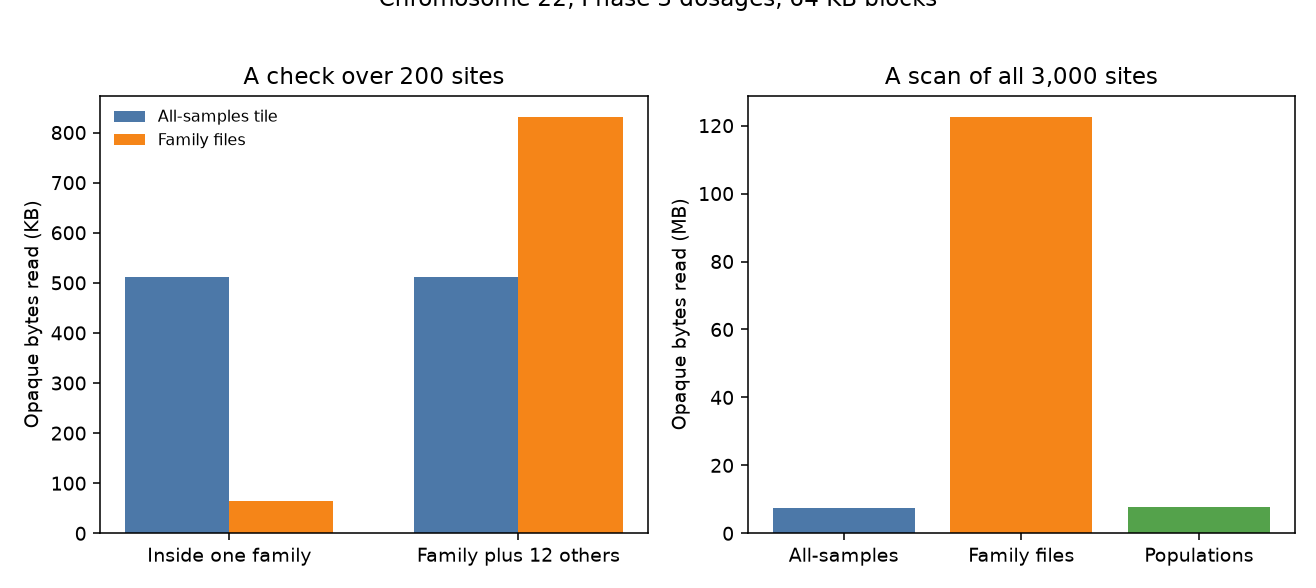
\includegraphics[width=\textwidth]{real_slice.png}
  \caption{Phase 3 chromosome 22, first 3{,}000 biallelic sites, 2{,}504 samples.
  Left: a 200-site window.
  A check that stays inside one pedigree family reads one 64\,KB block.
  The all-samples tile reads 512\,KB.
  Adding 12 people from outside that family reads 852\,KB, and the rule keeps the all-samples tile.
  Right: a scan.
  The family files read 123\,MB because each small file rounds up to a block.
  The five superpopulation files read 7.7\,MB, next to 7.5\,MB for one tile.}
  \label{fig:real}
\end{figure}

A check inside one superpopulation reads 188\,KB, and a check that names two superpopulations reads 366\,KB.
Both are below the 512\,KB all-samples window, so the rule keeps the population partition for those checks and drops it for a scan, where the population files read 7.7\,MB against 7.5\,MB.
The family partition is the one that flips inside a selective workload.
It wins for a check that stays in the family and loses as soon as the check picks up 12 other people, before any scan is added.

An uncompressed Parquet file of the same matrix, asked for the samples in one of those families over the same 200 sites, opens 325 bytes of column chunks.
Naming the samples removes the block.
The 8$\times$ gap between the family file and the all-samples tile is the opaque reader.
It is smaller than the simulator's 16$\times$ because a family of two to four people over 200 sites is below one 64\,KB block, so the read cannot shrink past that block.

The high-coverage panel of the same chromosome puts those missing relatives back~\cite{byrska2022}.
The file has 3{,}202 samples.
Of the first 3{,}290 variant rows, 3{,}000 are biallelic SNVs.
602 children have both parents in the callset, in 597 nuclear families.
Stored slots divided by samples equal 1.001, so a person is almost never kept twice.
The inside check is the first of those families, three people, over 200 sites, one byte per dosage.

At 64\,KB the all-samples window is 655{,}360 bytes, ten blocks, and the trio is 65{,}536 bytes, one block.
Adding twelve people from outside that trio opens thirteen blocks, 851{,}968 bytes, which is more than the all-samples window, so the rule does not keep the family files.
At 128\,MB the trio and the all-samples window are each one block of 134{,}217{,}728 bytes.
The $16$--$18\times$ figure stays the scaled simulator.
This callset does not reproduce it, and the near-unit duplication does not test the overlapping-parent penalty.

\section{Beyond a static cohort}
\label{sec:extensions}

The search in Section~\ref{sec:method} fixes the groups, then writes them.
The four counts in this section change one piece of that assumption at a time: arrivals that continue, a store that must not be given the edge list, a second payload with its own grouping, and a read that returns columns instead of whole blocks.
Each count uses synthetic ids.
Figure~\ref{fig:extensions} collects them.
None of the four is the eight-node sheet in Section~\ref{sec:lab}.

\begin{figure}[t]
  \centering
  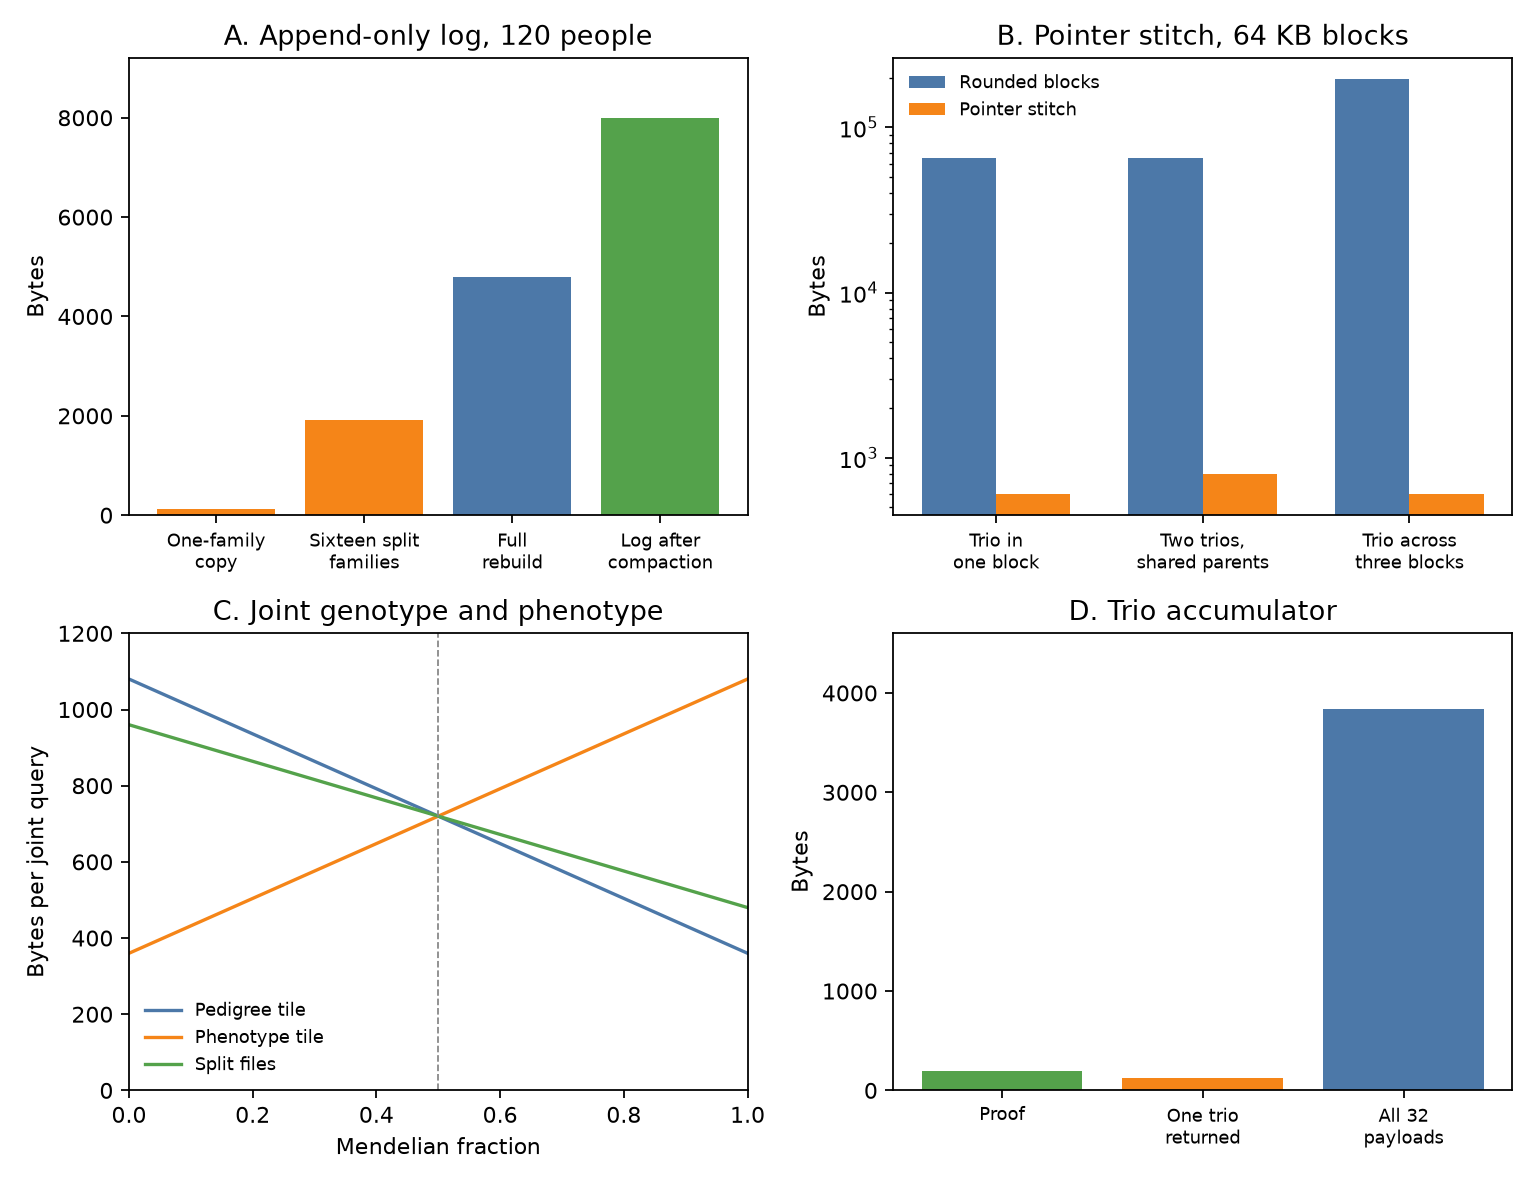
\includegraphics[width=\linewidth]{extensions.png}
  \caption{Synthetic layout counts.
  (A)~An append-only log of 120 people, 40 bytes each, 200-byte blocks.
  One split family copies 120 bytes.
  Sixteen split families copy 1{,}920 bytes of payload.
  One packed rebuild is 4{,}800 bytes, and the log is 8{,}000 bytes after the old runs are kept.
  (B)~Pointer stitch against 64\,KB rounding, 200-byte columns, log scale.
  (C)~Joint genotype and phenotype bytes on the nine-person orthogonal instance.
  The three layouts meet at Mendelian fraction \(1/2\).
  (D)~A Merkle check of 32 trio commitments returns one 120-byte payload.
  The proof is 192 bytes.
  The other payloads stay unopened.}
  \label{fig:extensions}
\end{figure}

\subsection{Append-only family log}
\label{sec:lsm}

New samples enter an open tail.
A full tail is sealed as an immutable level-0 run, in the sense of a log-structured merge tree~\cite{oneil1996lsm}.
A child does not copy parents who are already stored.
A trio check follows the alias of each person.
When the father, the mother, and the child occupy more than one block, compaction appends a level-1 run that holds only that family and swings those aliases.
Older runs stay on the log.
The caller flushes and compacts.
The measurement is the byte counter on that procedure.

Forty founder pairs arrive, then one child each: \(N = 120\) people, \(b = 40\) bytes per person, block size \(B = 200\).
Sealing the tail writes
\[
B_{\mathrm{flush}} = N b = 4800
\]
bytes, the same as one packed rebuild, and the compaction payload is still zero.
Sixteen of the forty trios cross a block boundary.
Compaction of one such family copies
\begin{equation}
W(F) = |F| \, b = 3 \times 40 = 120
\label{eq:family-copy}
\end{equation}
bytes.
The sixteen copies move \(16 \times 120 = 1920\) bytes of payload.
Each copy is sealed into its own block, so the log grows by \(\lceil 120 / 200 \rceil \times 200 = 200\) bytes per family:
\begin{equation}
B_{\mathrm{log}}
  = B_{\mathrm{flush}}
  + \sum_{F \in \mathcal{S}} \left\lceil \frac{|F| b}{B} \right\rceil B
  = 4800 + 16 \times 200
  = 8000.
\label{eq:lsm-log}
\end{equation}
One family copy is smaller than the rebuild.
The retained log is larger than the rebuild, because the level-0 bytes are not deleted when the aliases move.
A later sibling of a compacted family appends to the tail and leaves the sealed parents where they are.
That check is the third test of the log.

\subsection{Trio accumulator}
\label{sec:accum}

The planner keeps the HMAC key and the parent links~\cite{rfc2104}.
The store receives a Merkle root and one opaque payload per trio~\cite{merkle1987}.
A sample id \(i\) becomes the token \(\tau_k(i)\), the first 32 hex characters of \(\mathrm{HMAC}\text{-SHA256}(k, i)\).
The leaf of a trio is the SHA-256 hash of the three tokens in sorted order, under a fixed domain prefix, so the leaf does not record which member is the parent.
Parent hashes use a different domain prefix.
For a full tree of 32 leaves the membership proof is the leaf plus five sibling hashes,
\begin{equation}
|\pi| = 32 \times (1 + \log_2 32) = 192
\label{eq:proof}
\end{equation}
bytes.
The store returns the payload only when the sibling path recomputes the published root.
A one-bit change in the first sibling is rejected, and so is a leaf built with a different key.

On 32 trios with 120-byte payloads the accepted fetch returns 120 bytes.
The other 31 payloads are not opened.
The published document is 10{,}072 bytes.
It contains no kinship word, and it does not contain the HMAC tokens.
The document is larger than \(32 \times 120\) raw payload bytes because each payload is hex-encoded.
The query presents the leaf that is opened, so the store learns which commitment was fetched.
A planner that holds \(k\) can recompute every token.
The check does not evaluate the dosage bytes under encryption.

\subsection{Genotype tiles and phenotype tiles}
\label{sec:hyper}

A second payload needs its own grouping.
The genotype groups are three disjoint trios on nine ids,
\((0,1,2)\), \((3,4,5)\), and \((6,7,8)\).
Each id also carries a coordinate in \(\{e_1, e_2, e_3\}\), one standard basis vector, assigned so that the same axis appears in every trio.
Cosine similarity at threshold \(1/2\) links two ids when their coordinates match.
The phenotype components are then \((0,3,6)\), \((1,4,7)\), and \((2,5,8)\).
These coordinates are the input of the count.
No clinical note was embedded.

A hyper-tile stores both payloads for the people in one component.
Genotype payload is \(g = 100\) bytes and phenotype payload is \(p = 20\) bytes, so an opened component of size \(s\) costs \(s(g+p) = 120s\) bytes.
The split layout keeps genotypes in the pedigree groups and phenotypes in the similarity components, and a joint query opens both.
Let \(h\) be the fraction of queries that name one pedigree trio.
The rest name one phenotype component.
On this instance the three joint costs are linear:
\begin{equation}
\begin{aligned}
C_{\mathrm{ped}}(h) &= 360h + 1080(1-h) = 1080 - 720h, \\
C_{\mathrm{phe}}(h) &= 1080h + 360(1-h) = 360 + 720h, \\
C_{\mathrm{split}}(h) &= 480h + 960(1-h) = 960 - 480h.
\end{aligned}
\label{eq:joint}
\end{equation}
The 360-byte term is one component of three people.
The 1{,}080-byte term is all three components, which is what a query pays when the named ids cut across the grouping.
The split's 480 bytes are the pedigree genotypes of one trio, \(3 \times 100\), plus three phenotype components, \(3 \times 3 \times 20\).
Its 960 bytes are one phenotype component, \(3 \times 20\), plus three pedigree groups, \(3 \times 3 \times 100\).

\begin{proposition}
\label{prop:tiles}
On the joint costs~\eqref{eq:joint}, the pedigree tile is strictly cheaper for \(h > 1/2\), the phenotype tile is strictly cheaper for \(h < 1/2\), and all three layouts cost 720 bytes at \(h = 1/2\).
On a one-payload query the split layout costs \(60 + 240h \le 300\), while both hyper-tiles cost at least 360, so the split is strictly cheaper for every \(h \in [0,1]\).
\end{proposition}

\begin{proof}
Subtract the joint costs:
\(C_{\mathrm{ped}} - C_{\mathrm{phe}} = 1440(\tfrac12 - h)\) and
\(C_{\mathrm{ped}} - C_{\mathrm{split}} = 240(\tfrac12 - h)\),
so the pedigree tile is the unique minimum for \(h > 1/2\).
The symmetric difference \(C_{\mathrm{phe}} - C_{\mathrm{split}} = 600(2h - 1)\) makes the phenotype tile the unique minimum for \(h < 1/2\).
At \(h = 1/2\) each expression equals 720.
For a one-payload query the pedigree file is charged only \(g\) and the phenotype file only \(p\), which gives \(300h + 60(1-h) = 60 + 240h \le 300\).
Each hyper-tile still charges \(g+p\), and
\(C_{\mathrm{ped}}(h) - 360 = 720(1-h) \ge 0\),
\(C_{\mathrm{phe}}(h) - 360 = 720h \ge 0\).
\end{proof}

The measured fractions agree with the proposition: at \(h = 0.8\) the joint mix selects the pedigree tile (504 bytes), at \(h = 0.2\) it selects the phenotype tile (504 bytes), and at \(h = 0.5\) the three joint costs tie.
The one-payload mix selects the split at all three fractions, at 252, 180, and 108 bytes.

\subsection{Pointer stitch}
\label{sec:pointers}

Section~\ref{sec:inequality} charges a whole block for every byte range the query opens.
A pointer pool stores each column once and records parent ids on the child.
The stitch of a query \(Q\) is the unique columns,
\begin{equation}
T(Q) = |U(Q)| \, b,
\label{eq:stitch}
\end{equation}
and the block path charges every block those columns touch,
\begin{equation}
R(Q) = |\mathrm{blocks}(Q)| \, B,
\label{eq:rounded}
\end{equation}
including a short tail.
Columns are 200 bytes, the window width of the public-callset check, and \(B = 64\,\mathrm{KB}\).

Three adjacent columns sit in the first block, so \(R = 65536\) and \(T = 600\).
The same three people placed one in each of three blocks give \(R = 3 \times 65536 = 196608\) and the same stitch.
Two trios that share both parents store \(4 \times 200 = 800\) bytes.
Copying each trio into its own buffer writes \(6 \times 200 = 1200\) bytes.
The stitch of both children returns 800 bytes and does not allocate the extra copy.
The same gap appears on the small blocks used to test the pool: a three-column read rounds to 512 bytes against a 300-byte stitch, and three columns in separate 200-byte blocks round to 600 against 300.
The count is the byte difference~\eqref{eq:rounded} minus~\eqref{eq:stitch}.
No memory expander was attached, so the difference is not a device latency.

\subsection{The stitch on the high-coverage panel}
\label{sec:stitch-real}

The same formulas were then applied to the high-coverage chromosome~22 dosages, the first 3{,}000 biallelic SNVs and all 3{,}202 samples.
Each column is the vector of counted alleles for one sample.
Columns are packed in VCF order into 64\,KB blocks, and the short tail of a block is padded out to the block.
The stitch is the three columns of the first nuclear family with a sequenced child.
Those three people fall in one block.
Reads bypass the file cache with \texttt{FILE\_FLAG\_NO\_BUFFERING}.
The time is the median of seven trials after one warmup read, on the disk of this machine.

\begin{table}[t]
  \centering
  \caption{Pointer stitch on the high-coverage chromosome~22 panel.
  The trio is three people in one 64\,KB block.
  The aligned stitch read is 4{,}096 bytes at 200 sites and 12{,}288 bytes at 3{,}000 sites.}
  \label{tab:stitch}
  \small
  \setlength{\tabcolsep}{4pt}
  \begin{tabular}{@{}lrrrr@{}}
    \toprule
    & \multicolumn{2}{c}{200 sites} & \multicolumn{2}{c}{3{,}000 sites} \\
    \cmidrule(lr){2-3} \cmidrule(lr){4-5}
    Read & Bytes & ms & Bytes & ms \\
    \midrule
    Stitch & 600 & 0.160 & 9{,}000 & 0.108 \\
    One block & 65{,}536 & 0.331 & 65{,}536 & 0.168 \\
    Packed file & 655{,}360 & 0.454 & 10{,}027{,}008 & 7.45 \\
    \bottomrule
  \end{tabular}
\end{table}

At 3{,}000 sites the stitch is 9{,}000 bytes, the block that already holds the trio is 65{,}536, and the packed file is 10{,}027{,}008.
The unbuffered times are 0.108\,ms, 0.168\,ms, and 7.45\,ms.
The stitch beats the monolithic file by about \(69\times\) in time.
Against the one block that contains the trio, the byte ratio is \(65536/9000 \approx 7.3\) and the time ratio is about \(1.6\), because both reads are a single I/O.
At 200 sites the packed file is only ten blocks, and the three times sit between 0.160\,ms and 0.454\,ms.
Figure~\ref{fig:stitch} shows the 3{,}000-site bytes.
The synthetic placement that puts the three people in three different blocks, \(R = 196608\), does not occur for this trio.
VCF order already put them together.

\begin{figure}[t]
  \centering
  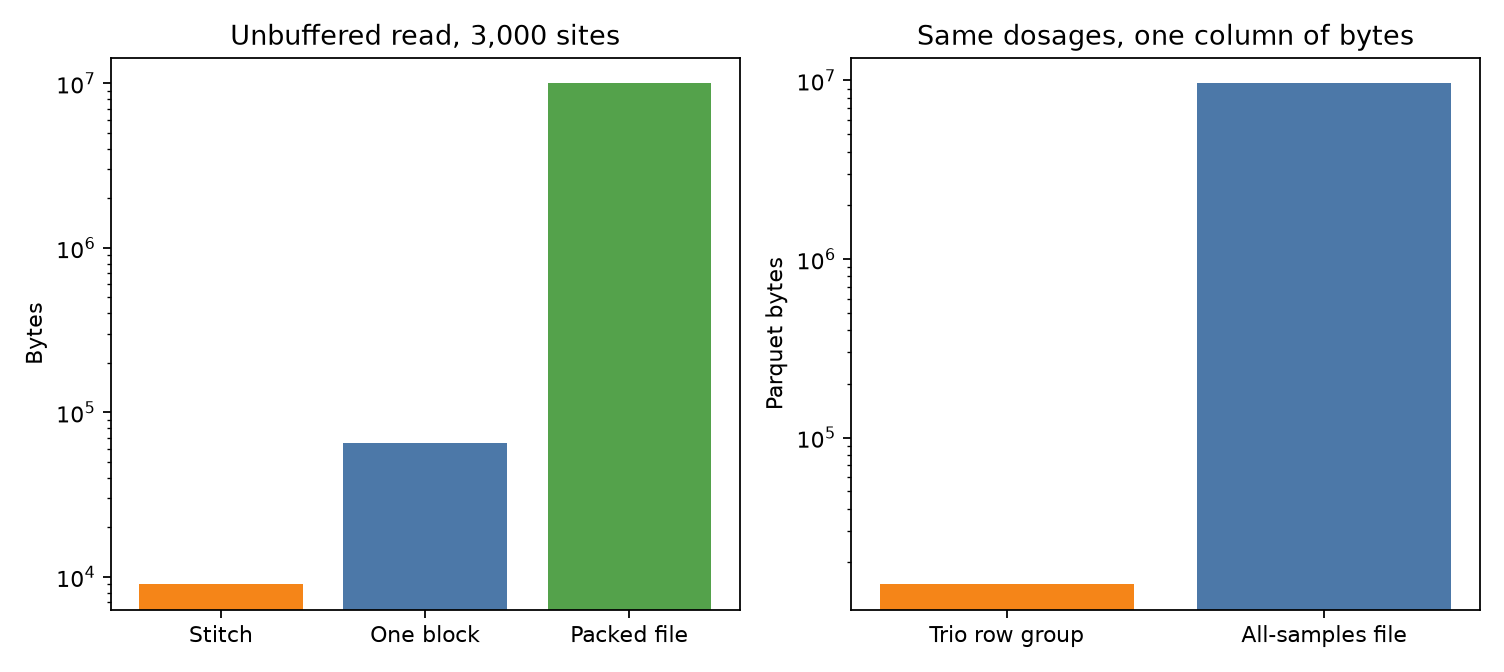
\includegraphics[width=\linewidth]{real_stitch.png}
  \caption{High-coverage chromosome~22, first 3{,}000 biallelic sites, one real trio.
  Left: unbuffered bytes for the stitch, the 64\,KB block that holds the three columns, and the packed file.
  Right: uncompressed Parquet. The trio is one row group of 15{,}069 bytes.
  The all-samples file is one row group of 9{,}644{,}279 column bytes.}
  \label{fig:stitch}
\end{figure}

\subsection{Where a withdrawn sample sits}
\label{sec:withdraw}

A duplicated tile is a second place a sample's bytes can remain after a consent withdrawal.
The pointer names the blocks that hold the sample, so the rewrite can be limited to those blocks.
On the 3{,}000-site packing the parent of the measured trio occupies one block.
Replacing that block writes 65{,}536 bytes.
Replacing the packed file writes 10{,}027{,}008.
Both flushes were timed on this disk, median of seven trials: 37.7\,ms for the block and 22.2\,ms for the file.
The alias cuts the bytes that must change.
At this file size it did not cut the flush time.

Three of the 3{,}202 people sit in two nuclear groups, and both groups have sizes 4 and 3.
A family-tile layout keeps both copies.
Deleting one of those people rewrites both groups.
Rounded to 64\,KB, that is 131{,}072 bytes, against the single block named by the pointer.
The other 3{,}199 people occupy one group.
The append-only log does not erase a sealed run.
A withdrawal appends a tombstone, the alias stops pointing at the old slot, and compaction rewrites the runs that still contain the sample.
Backups, query logs, and tables derived from the genotypes sit outside the alias.
The alias is the storage map for a withdrawal.
It is not, by itself, a decision that a deployment satisfies GDPR.

\subsection{The same groups as Parquet row groups}
\label{sec:rowgroups}

PedPack chooses the groups.
A columnar file can store each chosen group as a row group, and a reader that can name a sample can project those rows.
On these 3{,}000 sites the matrix is one binary column, one row per sample, uncompressed Parquet.
One row group for every sample holds 9{,}644{,}279 column bytes in a file of 9{,}650{,}656 bytes.
A median read of that file takes 10.5\,ms.
The nuclear group of the measured trio, written as its own row group, holds 15{,}069 bytes, and a median read of that row group takes 0.755\,ms.
Writing all 2{,}006 family and singleton groups as row groups produces a file of 34{,}011{,}188 bytes, because each row group pays for its own pages.
The policy is allowed to refuse that cut, as it already refuses a family tile when the workload does not pay for it.
Named projection remains the reason a columnar reader escapes the opaque-block bill.
The row group is how the same pedigree groups shorten a scan that reads the groups it is given.

\section{Related work}
\label{sec:related}

CoHadoop co-locates HDFS blocks that share a locator so a join can skip a shuffle~\cite{eltabakh2011cohadoop}.
PedPack also co-locates related records.
The unit is a genotype tile, the relatedness is the pedigree, and the cost is allowed to refuse the co-location when scans and duplication make it expensive.
CoHadoop does not choose tile shape.

Trojan layouts pick a column layout per block for a declared workload~\cite{jindal2011trojan}.
The search here is that idea on the sample axis of a matrix, with overlapping groups billed as extra bytes rather than as a join key.

A Hail MatrixTable is partitioned by locus interval~\cite{hail}.
Filtering to a few samples still reads every sample in the opened partitions.
That is the all-samples layout in this paper.
ADAM~\cite{massie2013adam} and Glow put reads and variants on Spark in the same locus-major shape.
They standardize the schema.
They do not search a pedigree cost.
The search here can be the input to that schema.
Section~\ref{sec:rowgroups} stores the groups it chose as Parquet row groups and reads the trio group instead of the cohort file.

TileDB stores a dense array as tiles whose shape the user picks~\cite{papadopoulos2016tiledb}.
PedPack is a policy for the sample side of a dosage matrix when some queries name families and the groups overlap.
The array store does not supply that policy, and it does not decide when the overlap has become too expensive to store.

The log in Section~\ref{sec:lsm} uses the LSM rule that a sealed run is immutable~\cite{oneil1996lsm}.
The difference is the compaction key: a nuclear family, not a key range.
The accumulator in Section~\ref{sec:accum} is Merkle's hash tree~\cite{merkle1987} over HMAC tokens~\cite{rfc2104}.
The opened leaf is visible to the store.

\section{Eight-node sheet}
\label{sec:lab}

Theorem~\ref{thm:gap} does not depend on a particular cluster.
The eight-desktop run is the check that the same sign survives NameNode placement, disk, and a remote fraction that is counted rather than fixed at \(0.60\).
Eight machines, one DataNode each, replication 3, client on a DataNode.
The genotypes are the 3{,}202-sample high-coverage panel, chromosome 22, whose pedigree file lists the relatives removed from the Phase~3 unrelated callset.
Each row is filled from that run.
The dashes below are unmeasured.
They are not zeros, and the paper is not submitted while they remain dashes.

\begin{table}[t]
  \centering
  \caption{Eight-node HDFS sheet.
  Remote fraction is the share of opened blocks whose replicas do not include the client DataNode.
  Every numeric cell is pending.}
  \label{tab:lab}
  \small
  \setlength{\tabcolsep}{5pt}
  \begin{tabular}{@{}lcccccc@{}}
    \toprule
    Read & Block &
    \begin{tabular}{@{}c@{}}Family\\bytes\end{tabular} &
    \begin{tabular}{@{}c@{}}All-samples\\bytes\end{tabular} &
    Ratio &
    \begin{tabular}{@{}c@{}}Remote\\fraction\end{tabular} &
    \begin{tabular}{@{}c@{}}Family/all\\seconds\end{tabular} \\
    \midrule
    5\% families & 64\,KB & --- & --- & --- & --- & --- \\
    5\% families & 128\,MB & --- & --- & --- & --- & --- \\
    15\% families & 64\,KB & --- & --- & --- & --- & --- \\
    Crossing & 64\,KB & --- & --- & --- & --- & --- \\
    Scan & 64\,KB & --- & --- & --- & --- & --- \\
    Parquet & --- & --- & --- & --- & --- & --- \\
    \bottomrule
  \end{tabular}
\end{table}

The 64\,KB rows test whether the simulator's selective byte ranking still holds once some replicas are local.
The 128\,MB row tests Lemma~\ref{lem:blocks}: a short one-byte window is one block on both layouts, and the scaled window is the four-to-one count above rather than \(16\times\).
The crossing row and the scan row are where Theorem~\ref{thm:gap} says the family layout stops paying.
The Parquet row is the columnar reader on the same samples.
A ratio near 1 there means the opaque-block gap did not survive a reader that can name a sample.

\section{What this does not show}
\label{sec:limits}

The block model has no NameNode heap, no disk, and no scheduler noise.
The HDFS numbers in the tables above this section are Docker on one host.
Table~\ref{tab:lab} is the eight-node measurement and is empty.
This machine has 16\,GB of RAM.
Four isolated virtual machines were not started, and the cloud command-line tools were not available, so a 4--8 node EMR or Dataproc cluster was not run.
A failed DataNode is implemented in the simulator and was not failed on hardware.

The 1000 Genomes run on the Phase~3 pedigree uses that pedigree and simulated dosages.
Chromosome~22 of the high-coverage panel is a public genotype matrix with 602 complete trios and duplication 1.001.
The kinship term is checked against Zstandard, not against PBWT.
The scaled matrices use a byte-per-genotype factor so that a family tile spans several 64\,KB blocks.
They are not tens of gigabytes of stored genotypes, and they are not a terabyte cohort.
Section~\ref{sec:inequality} is the same trade-off with rounding removed, and it is where a 128\,MB block drops the 200-site public window to one block on both layouts.

A paper that stops at this simulator, this single-host Hadoop, and this local Hail timing should say so in the abstract.
We have.

The append-only log, the accumulator, and the orthogonal phenotype coordinates in Section~\ref{sec:extensions} remain synthetic counts.
The log retains old runs, so its 8{,}000 bytes exceed one packed rebuild even though one family copy is 120 bytes.
The accumulator publishes the leaf that was opened, and a holder of the key can recompute every token.
The phenotype groups are nine coordinates, not a corpus of clinical notes.
The pointer stitch in Section~\ref{sec:stitch-real} is the high-coverage panel on one local disk, with the file cache bypassed.
It is not a memory expander, and it is not the eight-node sheet.
The withdrawal flush in Section~\ref{sec:withdraw} moved fewer bytes and took longer than rewriting the packed file.

\section{Conclusion}

On family-scoped access over moderately overlapping pedigrees, a cost-model search selects family layouts, matches an exhaustive winner inside a fixed measurement budget, and beats the same search without pedigree identity.
The advantage is query seconds per sample.
Storage seconds per sample go the other way, by $1.08$--$1.15\times$ on the two-generation cohorts where the nuclear groups contain the trios.
Where an extended check crosses that partition, the shuffle makes the query cost per sample rise as well, and the search keeps all-samples.
The advantage shrinks when duplication reaches about 1.4 or the workload becomes a scan, and both rankers then keep all-samples.
That refusal is part of the result.
On the high-coverage chromosome~22 panel the same refusal appears without a simulated dosage: one 64\,KB block for a real trio against ten for the cohort, and the all-samples window once twelve outsiders are added.
At 128\,MB those two windows are the same block.
The policy chooses groups for whatever reader consumes them.
On a columnar reader that can name a sample, projection removes the opaque-block bill, and the same groups become row groups: 15{,}069 bytes for one real trio against 9{,}644{,}279 column bytes for the cohort.
On the packed opaque file the pointer stitch of that trio is 9{,}000 bytes and 0.108\,ms, against 10{,}027{,}008 bytes and 7.45\,ms for the file, because the three columns already share one 64\,KB block.
A withdrawal follows the alias to that block.
The log, the accumulator, and the phenotype coordinates remain synthetic counts, and the eight-node sheet is still empty.

\section*{Data availability}
The simulator, the one-host HDFS measurements, and the chromosome~22 script are in the project repository.
Phase~3 genotypes are the public file
\texttt{ALL.chr22.phase3\_shapeit2\_mvncall\_integrated\_v5a.20130502.genotypes.vcf.gz}
from the 1000 Genomes FTP, restricted here to the first 3{,}000 biallelic sites.
The pedigree is the complete-parent subset of \texttt{20130606\_g1k.ped}.
The sample panel is \texttt{integrated\_call\_samples\_v3.20130502.ALL.panel}.
The trio measurement uses the high-coverage chromosome~22 panel
\texttt{1kGP\_high\_coverage\_Illumina.chr22.filtered.SNV\_INDEL\_SV\_phased\_panel.vcf}
and \texttt{3202\_samples.pedigree\_info.txt}, restricted to the first 3{,}000 biallelic SNVs.
The stitch, the withdrawal alias, and the Parquet row groups read that high-coverage VCF, restricted to the first 3{,}000 biallelic SNVs.
The append-only log, the accumulator, and the phenotype coordinates are synthetic ids.

\printbibliography

\end{document}
